\providecommand{\main}{../../../..}
\documentclass[\main/dresen_thesis.tex]{subfiles}
\begin{document}
  \label{sec:colloidalCrystals:nanoparticle:vsm}
  \begin{figure}[tb]
    \centering
    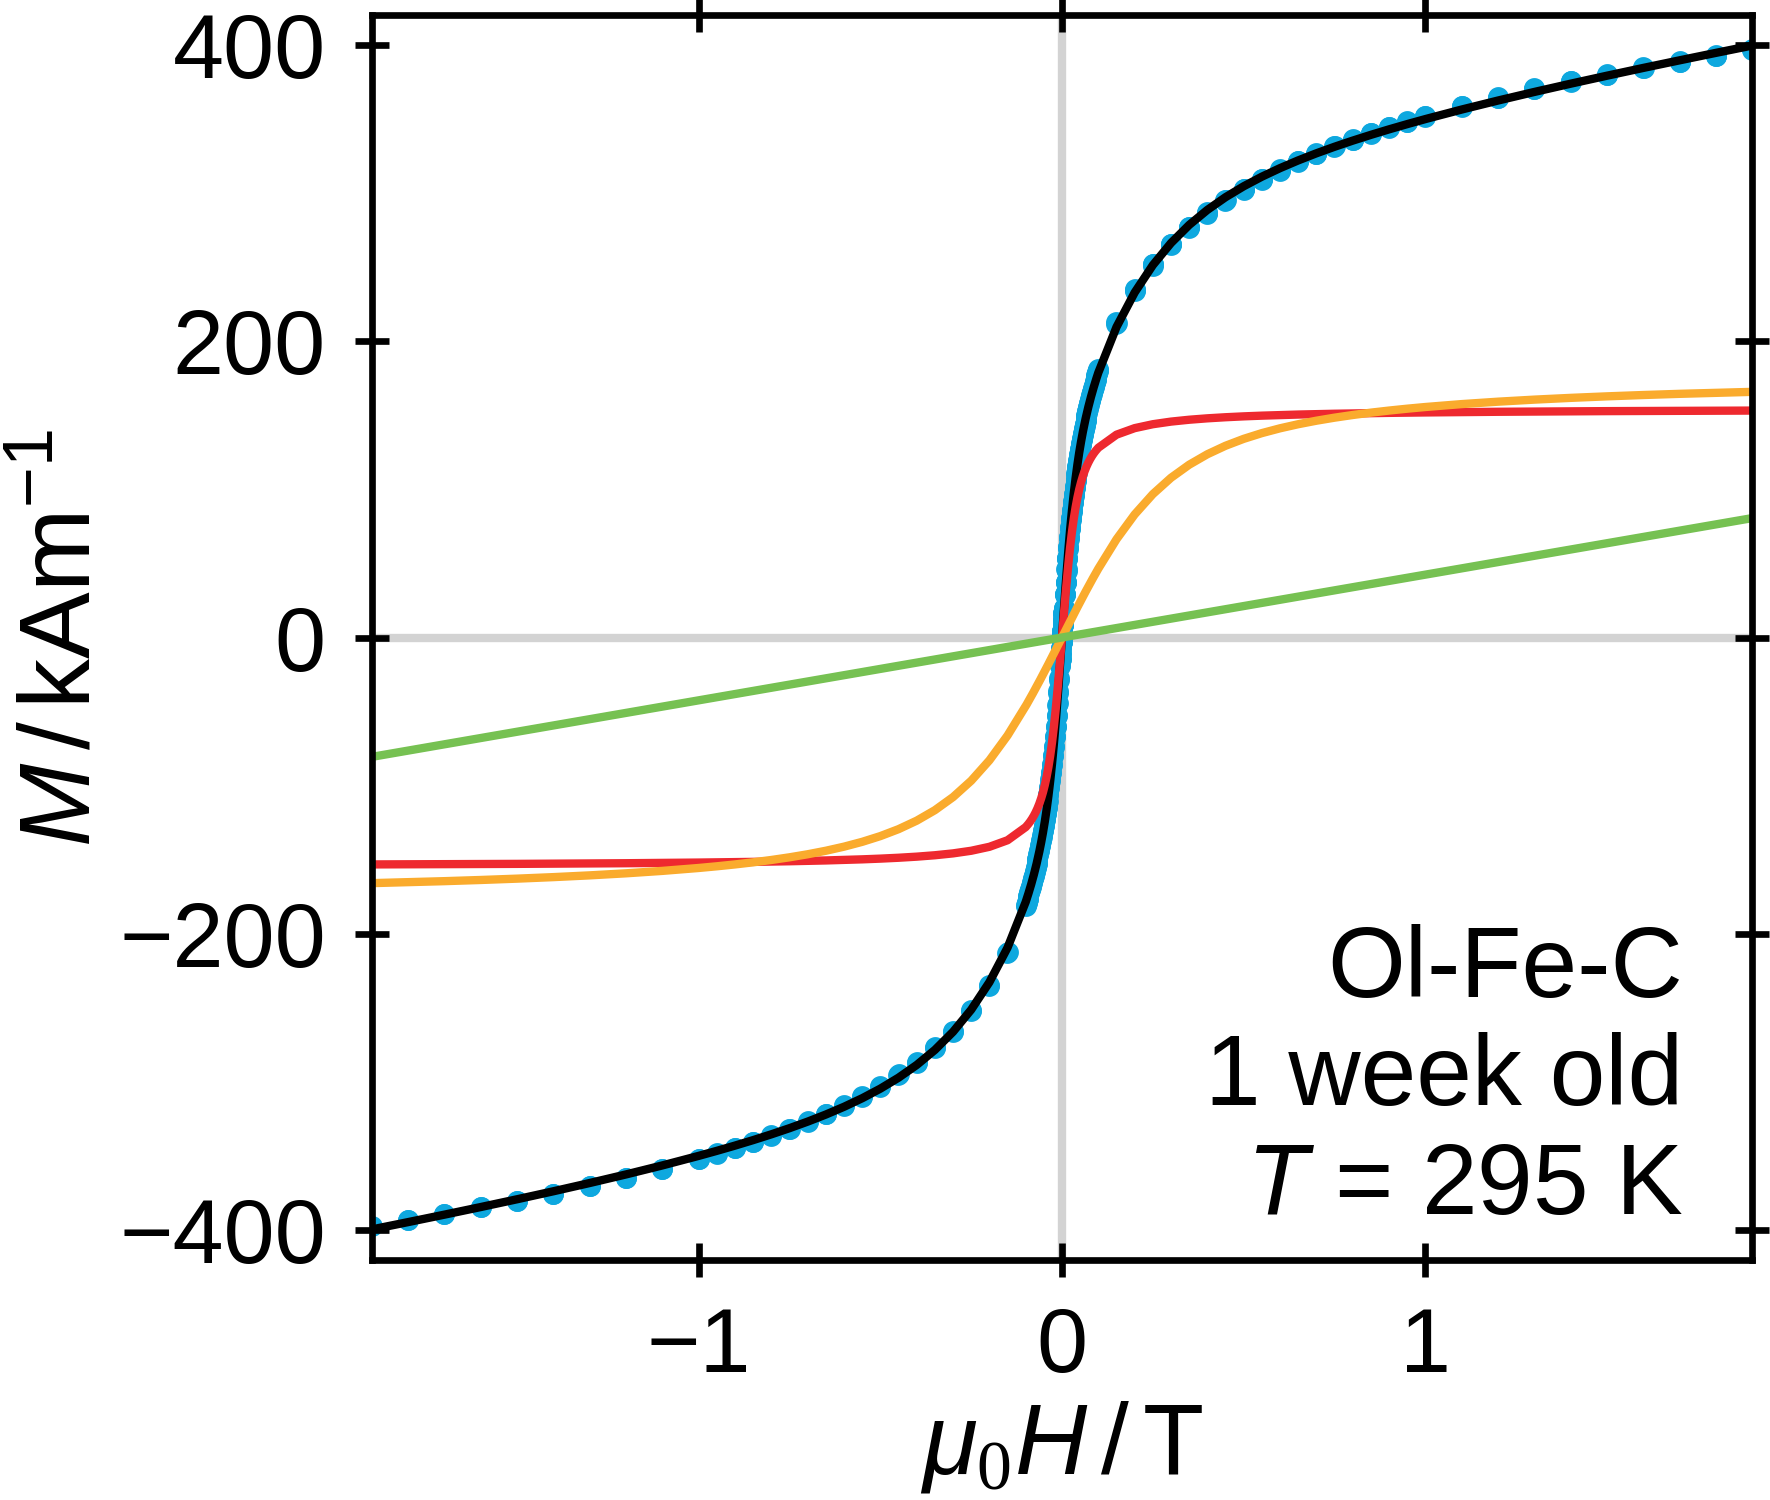
\includegraphics{colloidalCrystals_VSM_Ol_Fe_C}
    \caption{\label{fig:colloidalCrystals:nanoparticle:vsm}Room temperature VSM of Ol-Fe-C performed on a dry powder right after nanocube synthesis.}
  \end{figure}
  The magnetization of the nanocubes in a dry powder is shown in \reffig{fig:colloidalCrystals:nanoparticle:vsm} as measured within the week after synthesis.
  The obtained data from the powder deviates from a typical Langevin behaviour with excess susceptibility, as to why a linear combination of two Langevin behaviors and excess susceptibility is used to properly describe the data.
  The parameters of the best fit obtained by this model are tabulated in \reftab{tab:colloidalCrystals:nanoparticle:vsm}.

  \begin{table}[!htbp]
    \centering
    \caption{\label{tab:colloidalCrystals:nanoparticle:vsm} Fit parameters determined from the field-dependent magnetization measurements of the dried nanocubes at room temperature. A linear combination of two Langevin behaviour is fit, where $\mu_i$ is the single-particle magnetic moment and $M_{s,\,i}$ the spontaneous magnetization and $i\eq 1,\,2$ the two modes. $\chi$ is an additional excess susceptibility.}
    \begin{tabular}{ l | l }
      \rule{0pt}{2ex} \textbf{VSM @ 295 K} & Linear Comb. of Two Langevin \\
      \hline
      \rule{0pt}{2ex} $\mu_1 \, / \, \mu_B$                     & $25600(264)$\\
      \rule{0pt}{2ex} $\mu_2 \, / \, \mu_B$                     & $3605(65) $ \\
      \rule{0pt}{2ex} $M_{s,\,1} \, /  \unit{kA\,m^{-1}}$       & $155(1)$    \\
      \rule{0pt}{2ex} $M_{s,\,2} \, /  \unit{kA\,m^{-1}}$       & $177(1)$    \\
      \rule{0pt}{2ex} $\mu_0 \chi \, / \, 10^{-6}$              & $53300(900)$\\
      \hline
    \end{tabular}
  \end{table}

  A magnetic moment of $25600(264) \mu_B$ is determined for the first mode and a smaller moment of $3605(65) \mu_B$ for the second mode.
  With the total nanocube volume as determined by small-angle scattering, the first mode corresponds to nanoparticles with a spontaneous magnetization of $155(1) \unit{kA \, m^{-1}}$.
  With the thereby determined scale factor, the second mode has a spontaneous magnetization in a similar order of magnitude with $177 \unit{kA \, m^{-1}}$.
  The excess susceptibility is unusually large with an order of magnitude of $\mu_0 \chi \eq 53300 \cdot 10^{-6}$.
  A purely w\"ustite contribution would be expected in the order of $7200 \cdot 10^{-6}$ \cite{Lide_2004_Handb}.
  Possibly, the $\pm 2 \unit{T}$ range is not sufficient to properly determine the slope of the excess susceptibility, which results in this systematic error.

  The result from VSM reflects the core-shell structure of the nanocubes with a paramagnetic w\"ustite core and an inverse spinell shell, which is observed by the results from SAS and XRD.
  However, it has to be said that the performed VSM measurements are sub-optimal to characterize the non-interacting nanocube properties, as for one they were performed for a dry sample, where it was showed in \refsec{sec:monolayers:nanoparticle:vsm} that the magnetic properties of nanoparticles can greatly vary when comparing the diluted case and the dry state.
  For the other, due to the unstable phase of the nanocubes, it is difficult to compare the results across multiple complimentary experiments.
  An improved VSM study using nanocubes in a well-defined phase and within a well-diluted state is however out of the scope of this present thesis.
\end{document}
